\chapter{A ROBUST CONTROL SCHEME FOR AN INTEGRATED DUAL-OUTPUT UNIFIED POWER QUALITY CONDITIONER}
\label{6.Chap:DOCUPQC}
\section{INTRODUCTION}
In the preceding chapters, the limitations of the series converter in the unified power quality conditioner (UPQC) due to infrequent voltage-related issues in the distribution system (DG) have been explored. Consequently, the conventional back-to-back converter-based UPQC experiences reduced converter utilization. To address this issue and enhance converter utilization, a reduced switch count topology known as the dual-output converter (DOC) has been considered for UPQC application. The performance characteristics of the DOC and its control operation using linear controllers have been examined. In order to further improve performance of DOC based UPQC and ensure robustness against model inaccuracies and disturbances, a sliding mode controller (SMC) has been considered.

It has been emphasized that controlling the converter/load neutral-point voltage is essential for effectively controlling DOC-based systems. Additionally, implementing the complete control algorithm in the natural frame helps mitigate signal transformation errors and reduce computational burden to some extent. Taking all these factors into consideration, a new sliding surface-based SMC scheme has been proposed and independently evaluated on both the four-leg DSTATCOM and DVR. Since the UPQC integrates the functionalities of DSTATCOM and DVR, the proposed SMC scheme is applied to the DOC-based UPQC, and its performance is analyzed in this chapter under various grid conditions using MATLAB simulations. %\vspace*{2cm}
    
\begin{sidewaysfigure}[]   
	\centering
	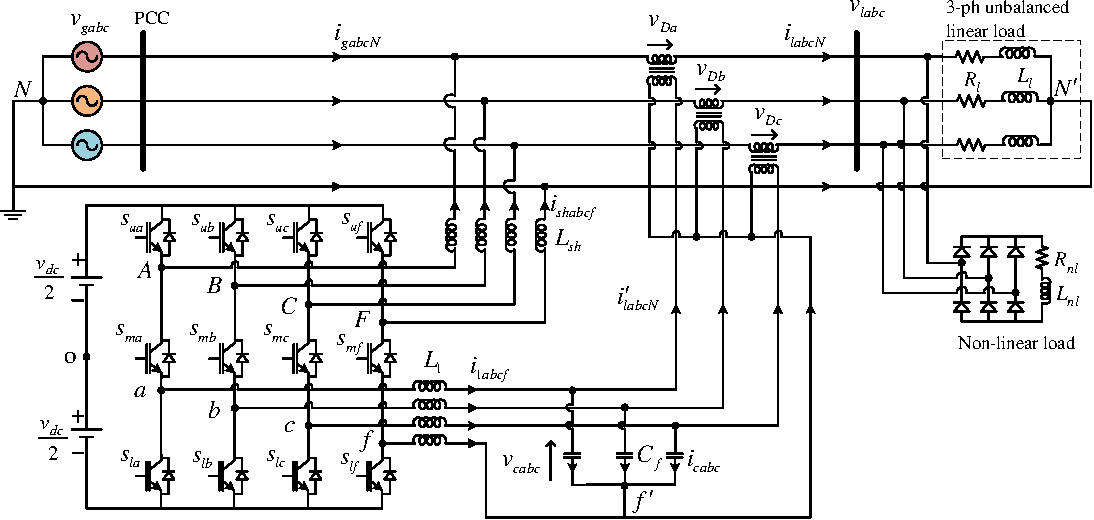
\includegraphics[scale=1]{figures/Chapter_6/Mine/4leg_UPQC_L.pdf}
	\caption{A dual output converter based UPQC-L}
	\label{fig6.1}
\end{sidewaysfigure}

\section{DESCRIPTION OF THE SYSTEM}
Fig.~\ref{fig6.1} illustrates the schematic of a three-phase four-wire distribution system incorporating a four-leg dual-output converter-based UPQC. The control algorithm developed for the DSTATCOM is applied to the upper terminals of the dual-output converter, while the control algorithm developed for the DVR is applied to the lower terminals of the DOC.

The system consists of both a three-phase balanced linear RL load and a non-linear load comprising a diode bridge rectifier with an RL load. The shunt compensator current $(i_{shabcf})$ is regulated by employing a shunt filter inductor $L_{sh}$, and the series compensator voltage $(v_{Dabc})$ is regulated using an LC filter comprising inductor $L_{1}$ and capacitor $C_{f}$. The dual-output converter is connected to a stiff DC source, assuming that the DC-link voltage does not exhibit any dynamics.

The notations and model equations introduced for the DSTATCOM in Chapter \ref{4.Chap:DSTATCOM} are used for the upper ports of the dual-output converter, while the notations and model equations introduced for the DVR in Chapter \ref{5.Chap:DVR} are used for the lower ports of the dual-output converter.

\section{PROPOSED CONTROL SCHEME}
The control algorithm consists of two main components: the generation of reference quantities, such as compensator currents, compensator voltages, and neutral-point voltages, and the implementation of a sliding mode controller. 
\begin{sidewaysfigure}[]   
	\centering
	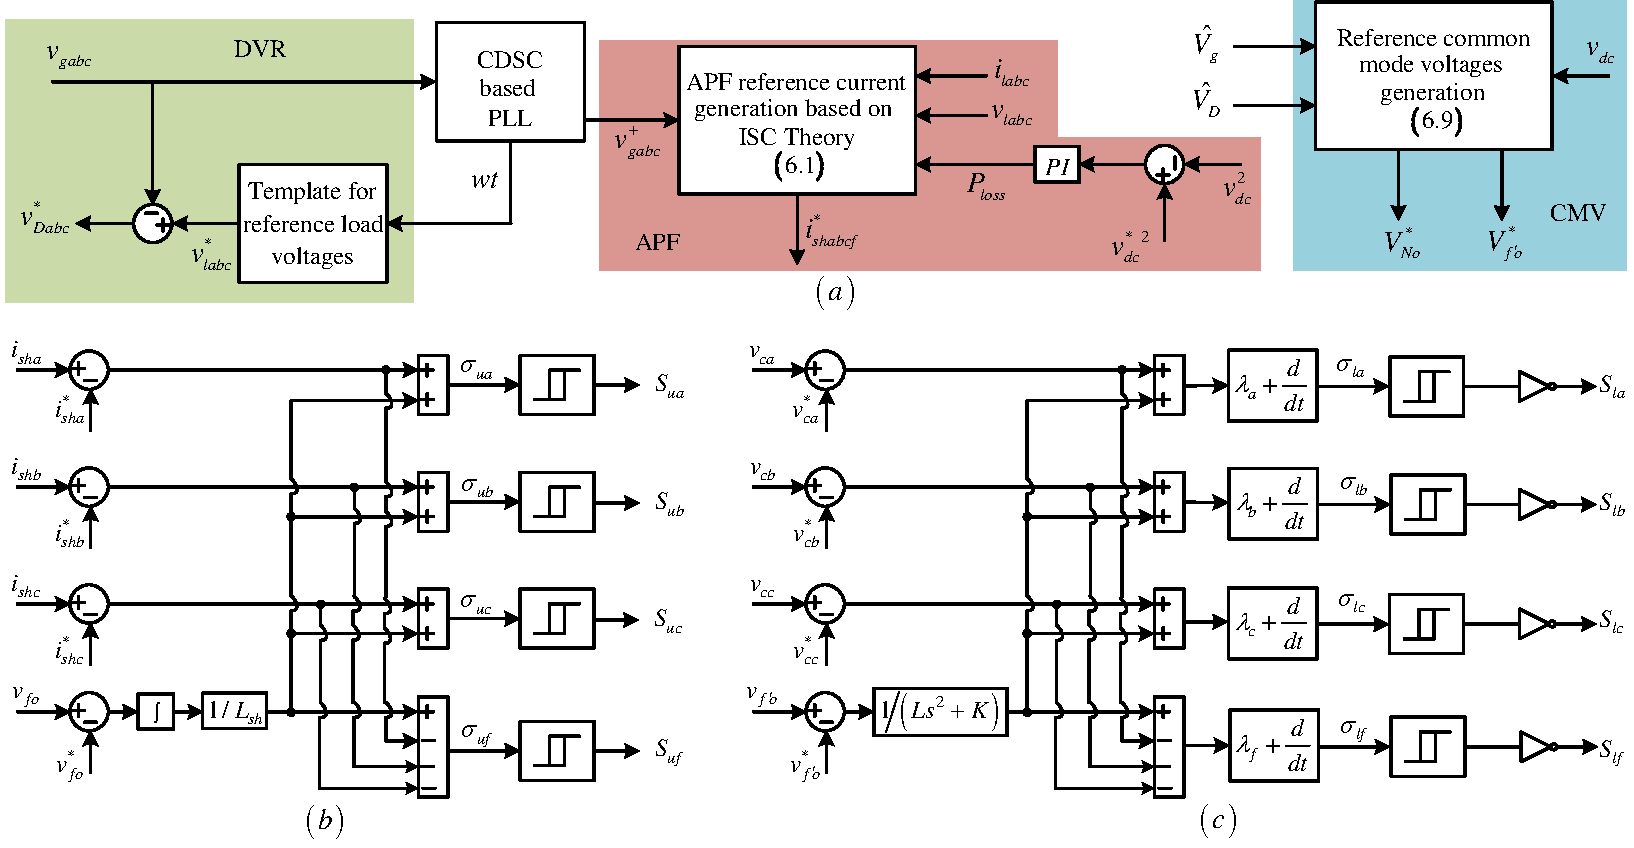
\includegraphics[scale=0.9]{figures/Chapter_6/Mine/Control_Diagram.pdf}
	\caption{Control schematics: (a) Reference generation, (b) Upper switches gating pulse generation, and (c) Lower switches gating pulse generation}
	\label{fig6.3}
\end{sidewaysfigure}

\subsection{Generation of Reference Quantities}
The complete block diagram of the required reference generations for sliding mode control are shown in Fig.\,\ref{fig6.3}(a). The reference currents for shunt APF are generated using instantaneous symmetrical component theory (ISCT) discussed in Chapter \ref{2.Chap:DOCIntro}. In order to achieve unity power factor operation at the grid, the variable $\gamma^+$ is substituted with zero in \eqref{eqn2.52}. The resultant expressions for the reference currents are as follows:  
\begin{equation} \label{6.20}
\begin{aligned}
i^{*}_{shi} &= i_{li} - \frac{v^{+}_{gi}}{\sum_{k=a,b,c}^{}\left(v^{+}_{gk}\right)^{2}} \left(P_{lavg} + P_{loss}\right) \hspace{1.5cm} \forall ~~ i ~ \epsilon ~ \{a,b,c\}, \\
i^{*}_{shf} &= - \sum_{i = a,b,c} i^{*}_{shi},
\end{aligned}
\end{equation}
where, $P_{lavg}$ and $P_{loss}$ are average load power and converter power losses respectively. The fundamental positive sequence components of grid voltages, $v^{+}_{gj}$ are extracted using CDSC operator. The converter power loss component is found from the mismatch in the DC-link voltage with its reference voltage using linear PI controller. The gains of controller are computed based on fast acting DC-link voltage controller, ensuring a rapid transient response \cite{5235863}. It is worth noting that when a stiff DC source is utilized, the PI controller is not necessarily required. However, it is included in Fig.\,\ref{fig6.3}(a) for general understanding. 

For the extraction of the grid voltage angle, a phase-locked loop (PLL) based on the CDSC operator, proposed in \cite{6276263}, is employed. This PLL offers superior performance compared to the commonly used second order generalized integrator (SOGI) based PLL, as discussed in Chapter \ref{3.Chap:PLL}. By utilizing the extracted phase angle, a reference template for load voltages is defined. The DVR reference voltages are then generated by subtracting the grid voltages from the defined load voltage template. The expression for DVR reference voltages based on the in-phase compensation scheme is defined as follows:
\begin{equation} \label{6.2}
\begin{aligned}
v^{*}_{Di} = v^{*}_{li} - v_{gi} \hspace{1.5cm} \forall ~~ i ~ \epsilon ~ \{a,b,c\}.
\end{aligned}
\end{equation}

In Chapter \ref{2.Chap:DOCIntro}, it was discussed that offsets are added to both the modulating signals of the upper port and the lower port in order to avoid any intersection between the two modulating signals. Additionally, the offset ensures that the upper modulating signal is always higher than the lower modulating signal. These offsets contribute to the control of the respective neutral-point voltages (NPVs).

To gain a better understanding of this concept and to derive expressions for the reference quantities of the NPVs, the pulse width modulation (PWM) requirements for the DOC based UPQC-L are presented in Fig.\,\ref{fig6.2}. In the case of the UPQC-L, the upper port is utilized for DSTATCOM operation, and its voltage is approximately the same as the voltage at the point of common coupling (PCC). Hence, the modulating signal of the upper port is represented as $v_g$ in Fig.\,\ref{fig6.2}. On the other hand, the lower port of the UPQC-L is employed for DVR operation, and its voltage is the difference between the desired load voltage ($v^{*}_{l}$) and the PCC voltage ($v_{g}$). Consequently, the modulating signal of the lower port is denoted as $v_{D}$ in Fig.\,\ref{fig6.2}. The offsets or reference NPVs are added to these modulating signals to satisfy the following conditions, which ensure the generation of valid switching states for the DOC-based UPQC-L system.
\begin{figure}[]   
	\centering
	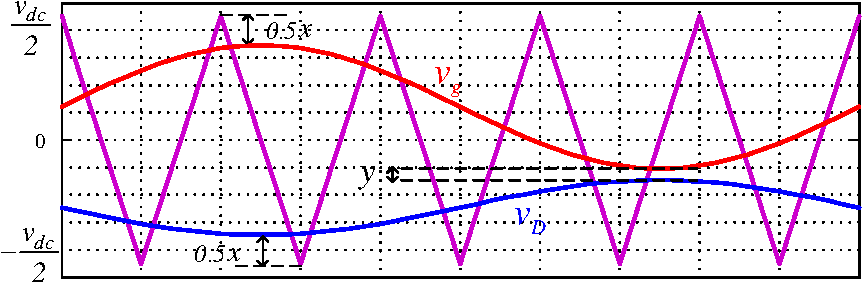
\includegraphics[scale=1]{figures/Chapter_6/Mine/NPV_Calculations.pdf}
	\caption{Illustration of PWM logic of DOC based UPQC-L for reference NPV calculations}
	\label{fig6.2}
\end{figure}
\begin{enumerate} \vspace*{-0.4cm}
	\item Ensuring that the positive peak of the upper modulating signal is within the positive peak of the carrier signal, thus avoiding over modulation issues. This can be mathematically stated as follows: \vspace*{-0.4cm}
	\begin{equation}  \label{6.3}
	\begin{aligned}
		V^{*}_{No} + \hat{V}_{g} \leq \frac{v_{dc}}{2}, \\
		\Rightarrow V^{*}_{No} = \frac{v_{dc}}{2} - \hat{V}_{g} - \frac{x}{2},
	\end{aligned}
	\end{equation}
	where $V^{*}_{No}$ represents the reference NPV for upper port, $\hat{V}_{g}$ represents the positive peak of the grid/PCC voltage, and $x$ represents the sum of free space available between the positive peak of upper modulating signal and positive peak of carrier signal, as well as the free space available between the negative peak of lower modulating signal and the negative peak of carrier signal. In Fig.\,\ref{fig6.2}, it is assumed that the free space at the positive peak of carrier is same as the free space at the negative peak of the carrier.
	
	\item Ensuring that the negative peak of the lower modulating signal is within the negative peak of the carrier signal, thereby avoiding over modulation issues. This can be mathematically stated as follows:
	\begin{equation}  \label{6.4}
	\begin{aligned}
	V^{*}_{f^{\prime}o} - \hat{V}_{D} \geq -\frac{v_{dc}}{2}, \\
	\Rightarrow V^{*}_{f^{\prime}o} = -\frac{v_{dc}}{2} + \hat{V}_{D} + \frac{x}{2},
	\end{aligned}
	\end{equation}
	where $V^{*}_{f^{\prime}o}$ represents the reference NPV for lower port, and $\hat{V}_{D}$ represents the absolute/positive peak of the DVR voltage reference. 
	
	\item Ensuring that the upper modulating signal is always higher than the lower modulating signal. This can be realized mathematically as given below:
	\begin{equation}  \label{6.5}
	\begin{aligned}
	V^{*}_{No} - \hat{V}_{g} \geq V^{*}_{f^{\prime}o} + \hat{V}_{D}, \\
	\Rightarrow V^{*}_{No} = V^{*}_{f^{\prime}o} + \hat{V}_{D} + \hat{V}_{g} + y,
	\end{aligned}
	\end{equation}
	where $y$ represents the free space between the negative peak of upper modulating signal and the positive peak of the lower modulating signal. This space can be as low as possible compared to the space $x$. In this study, $y$ is considered as $0.2$ times the value of $x$, i.e.,
	\begin{equation}  \label{6.6}
		y = 0.2 \, x.
	\end{equation} 
\end{enumerate}

By substituting \eqref{6.3} and \eqref{6.4} into \eqref{6.5}, the total free space can be obtained as below:
\begin{equation} \label{6.7}
x + y = v_{dc} - 2(\hat{V}_{g} + \hat{V}_{D}).
\end{equation}
By substituting \eqref{6.6} into \eqref{6.7}, the following is obtained:
\begin{equation} \label{6.8}
x = \frac{v_{dc} - 2(\hat{V}_{g} + \hat{V}_{D})}{1.2}.
\end{equation} 
Ensuring the positive values for free space is crucial. By substituting $ \hat{V}_{D} = | \hat{V}^*_{l} -  \hat{V}_{g}|$ into \eqref{6.8}, the range of compensation voltage that maintains a positive free space can be determined. The notation $\hat{V}^*_{l}$ represents the positive peak of the desired load voltage. The condition for achieving a positive free space is given as below.
\begin{equation} \label{6.14}
v_{dc} > 2(\hat{V}_{g} + | \hat{V}^*_{l} -  \hat{V}_{g}|)
\end{equation} 
During the voltage sag conditions, where $\hat{V}^*_{l} > \hat{V}_{g}$, the condition that needs to be satisfied is:
\begin{equation} \label{6.15}
v_{dc} > 2 \hat{V}^*_{l}.
\end{equation} 
Typically, the DC-link voltage is selected in a way that satisfies the above condition. This indicates that the DOC based UPQC can perform all of its functions satisfactorily during the voltage sag conditions. On the other hand, during the voltage swell conditions, where $\hat{V}^*_{l} < \hat{V}_{g}$, \eqref{6.14} is modified as below.
\begin{equation} \label{6.16}
\begin{aligned}
v_{dc} &> 2(\hat{V}_{g} + \hat{V}_{g} - \hat{V}^*_{l} ) \\
\frac{v_{dc}}{2} &> 2 \hat{V}_{g} - \hat{V}^*_{l} \\
\hat{V}_{g} &< \frac{0.5v_{dc} + \hat{V}^*_{l}}{2}
\end{aligned}
\end{equation} 
Therefore, the maximum voltage swell that can be compensated by the DOC based UPQC is $\frac{0.5v_{dc} + \hat{V}^*_{l}}{2}$.

The reference NPVs of upper port and lower port can be obtained by substituting \eqref{6.8} into \eqref{6.3} and \eqref{6.4}, respectively, as given below:
\begin{equation} \label{6.9}
\begin{aligned}
V^{*}_{No} &= \frac{1}{12}\Big\{ v_{dc} - 2\hat{V}_{g} + 10\hat{V}_{D} \Big\}, \\
V^{*}_{f^{\prime}o} &= \frac{1}{12}\Big\{ -v_{dc} - 10\hat{V}_{g} + 2\hat{V}_{D} \Big\}.
\end{aligned}
\end{equation}  

\subsection{Implementation of Proposed SMC}
The sliding variables proposed for DSTATCOM in Chapter \ref{4.Chap:DSTATCOM} and the sliding variables proposed for DVR in Chapter \ref{5.Chap:DVR} are redefined in this section. By substituting \eqref{4.4} into \eqref{4.8}, the sliding variables for the upper port of DOC based UPQC-L are defined as follows:
\begin{equation} \label{6.10}
%\begin{aligned}
\sigma_{uj} = (i_{shj} - i^{*}_{shj} ) + \frac{1}{L_{sh}} \int (v_{No} - v^{*}_{No}) \, dt; \hspace{0.5cm} \forall ~~ j ~ \epsilon ~ \{a,b,c,f\}. \\
%V^{*}_{f^{\prime}o} &= \frac{1}{12}\Big\{ -v_{dc} - 10\hat{V}_{g} + 2\hat{V}_{D} \Big\}
%\end{aligned}
\end{equation}

For each leg of the DOC in the upper port, there are four sliding variables. For phase-$a$ leg, the sliding variable, $\sigma_{ua}$ is considered and it is passed to a hysteresis modulator to generate switching pulses for the upper switch of DOC. When $\sigma_{ua}$ crosses the upper hysteresis band, the top switch $S_{ua}$ is turned OFF. Conversely, when $\sigma_{ua}$ crosses the lower hysteresis band, the top switch is turned ON. If $\sigma_{ua}$ is within the hysteresis band, the state of the switch remains unchanged. The same principle applies to the other legs of DOC. The complete implementation of SMC for the upper port of DOC based UPQC-L is shown in Fig.\,\ref{6.3}(b).

Similarly, by substituting \eqref{5.8} into \eqref{5.9}, the sliding variables for the lower port of DOC based UPQC-L can be defined as follows:
\begin{equation} \label{6.11}
%\begin{aligned}
\sigma_{lj} = \Big(\lambda_{j} + \frac{d}{dt} \Big) \Big\{ (v_{cj} - v^{*}_{cj}) + (v_{c\gamma} - v^{*}_{c\gamma}) \Big\}; \hspace{0.5cm} \forall ~~ j ~ \epsilon ~ \{a,b,c,f\}, \\
%V^{*}_{f^{\prime}o} &= \frac{1}{12}\Big\{ -v_{dc} - 10\hat{V}_{g} + 2\hat{V}_{D} \Big\}
%\end{aligned}
\end{equation}
where $v_{cf} = - \sum_{k = a,b,c} v_{ck}$, and $v^{*}_{cf} = - \sum_{k = a,b,c} v^{*}_{ck}$. The fictitious voltages ($v_{c\gamma}, v^{*}_{c\gamma} $) are obtained from \eqref{5.33}, which is given as below.
\begin{equation} \label{6.12}
V_{c\gamma}(s) = \frac{1}{Ls^{2} + K}\,V_{f^{\prime}o}(s)
\end{equation}
Where $L = L_1C_f$, and $K = (1 + \frac{L_{1}}{L_{t}} ) $.

For each leg of the DOC in the lower port, there are four sliding variables. For phase-$a$ leg, the sliding variable, $\sigma_{la}$ is considered and it is passed to a hysteresis modulator to generate switching pulses for the lower switch of DOC. When $\sigma_{la}$ crosses the upper hysteresis band, the bottom switch $S_{la}$ is turned ON. Conversely, when $\sigma_{la}$ crosses the lower hysteresis band, the bottom switch is turned OFF. If $\sigma_{la}$ is within the hysteresis band, the state of the switch remains unchanged. The same principle applies to the other legs of DOC. The complete implementation of SMC for lower port of DOC based UPQC-L is shown in Fig.\,\ref{6.3}(c). 

The switching state for the middle switches ($S_{mj}$) is obtained by performing NAND operation on the switching state of upper switches ($S_{uj}$) and lower switches ($S_{lj}$). This can be realized mathematically as follows:
\begin{equation} \label{6.13}
S_{mj} = \overline{S_{uj}\cdot S_{lj}} \hspace{1cm} \forall ~~ j ~ \epsilon ~ \{a,b,c,f\}.
\end{equation}

\section{SIMULATION STUDIES}
\begin{table}[] 
	\centering
	\captionof{table}{System parameters}
	\label{Table6.2}
	\begin{tabular}{>{\small}c>{\small}c}  
		\hline
		\hline
		\textbf{\footnotesize System parameters} & \textbf{\footnotesize Simulation values}\\
		\hline
		\footnotesize Rated supply phase voltage & \footnotesize$230 ~\si{V}, 50 ~\si{Hz}$ \\
		\footnotesize Filter parameters & \footnotesize $L_{sh} = 20 ~\si{mH}$, $L_{t} = 3 ~\si{mH}$ \\ & \footnotesize $L_{1} = 5 ~\si{mH}$, $C_{f} = 30 ~\si{\mu F}$ \\ 
		\footnotesize DC-link voltage & \footnotesize $v_{dc} = 900 ~\si{V}$ \\
		\footnotesize Sliding surface coefficients & \footnotesize $\lambda_i = 2582$, $\lambda_f = 4145$ \\
		\footnotesize Linear load  &  \footnotesize $Z_{a} = 200+j60\,\si{\Omega}$, \\ & \footnotesize $Z_{b} = 60+j55\, \si{\Omega}$, \\  & \footnotesize $Z_{c} = 30+j25\, \si{\Omega}$ \\
		\footnotesize Nonlinear load  &  \footnotesize $3$-$\phi$ diode bridge rectifier with \\ & \footnotesize $R_{nl} = 40  ~\Omega$ ~; ~ $L_{nl} = 0.5 ~\si{H}$ \\ 
		\footnotesize Injection transformer & \footnotesize 230\,\si{V}, 33\,\si{kVA}, turns ratio 1:1 \\
		\hline
		\hline 
	\end{tabular} \vspace*{-0.5cm}
\end{table}
The MATLAB/Simulink tool is used to model the four-leg dual output converter based UPQC shown in Fig.\,\ref{fig6.1}, along with the proposed sliding mode control. The simulation considers the system parameters listed in Table\,\ref{Table6.2}. Based on these parameters and \eqref{6.16}, the maximum voltage swell that can be compensated by the DOC-based UPQC is $387.5 \,$V (peak) or $1.1923$ pu. To validate the proposed control method, a simulation study is conducted for various grid voltage disturbances. Each event is considered for a duration of 0.06\,s to ensure visual clarity and accommodate all voltage-related events in a plot.

In Fig.\,\ref{6.Res1}, the occurrence of a balanced voltage sag ($V_{g} = 0.5\, \si{pu}$), an unbalanced voltage sag in phase-$a$ ($V_{ga} = 0.5\, \si{pu}$), and a balanced voltage swell ($V_{g} = 1.1\, \si{pu}$) are considered at 0.5\,s, 0.56\,s, and 0.62\,s, respectively. In Fig.\,\ref{6.Res2}, the occurrence of an unbalanced voltage swell in phase-$a$ ($V_{ga} = 1.1\, \si{pu}$), a balanced voltage swell ($V_{g} = 1.2\, \si{pu}$), and an unbalanced voltage swell in phase-$a$ ($V_{ga} = 1.2\, \si{pu}$) are considered at the time instants of 0.68\,s, 0.74\,s and 0.8\,s, respectively. All these voltage anomalies have a fundamental frequency component. A distorted grid is considered at time 0.86\,s as shown in Fig.\,\ref{6.Res2}. 
\begin{sidewaysfigure}[]\centering
	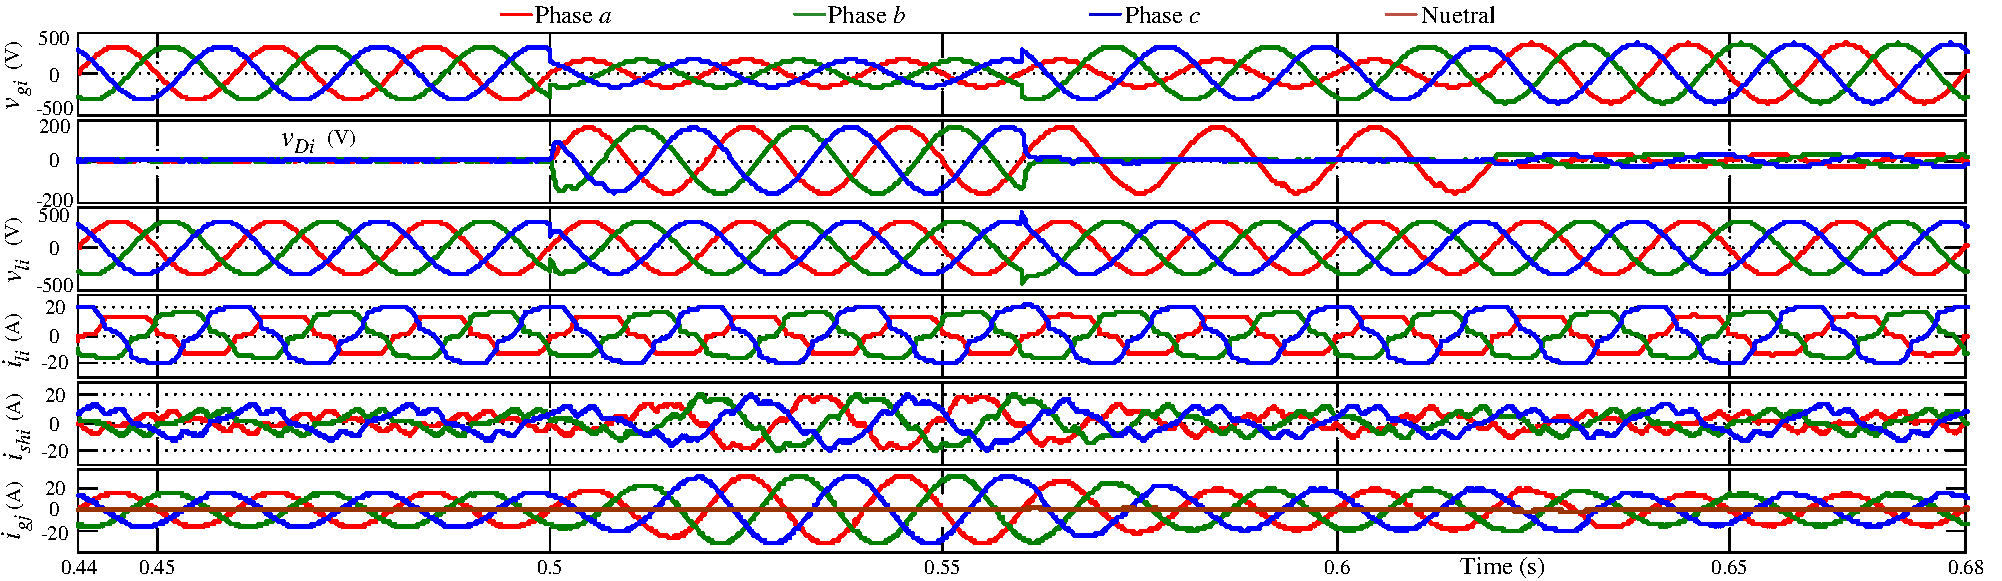
\includegraphics[scale=0.72	]{figures/Chapter_6/Mine/Res1.pdf}
	\caption{Simulation results of proposed SMC based four-leg DOC based UPQC-L during voltage anomalies with fundamental component: normal grid ($V_g = 1\,$pu), balanced sag ($V_g = 0.5\,$pu), unbalanced sag ($V_{ga} = 0.5\,$pu), and balanced swell ($V_g = 1.1\,$pu)} 
	\label{6.Res1} \vspace*{0.5cm}
	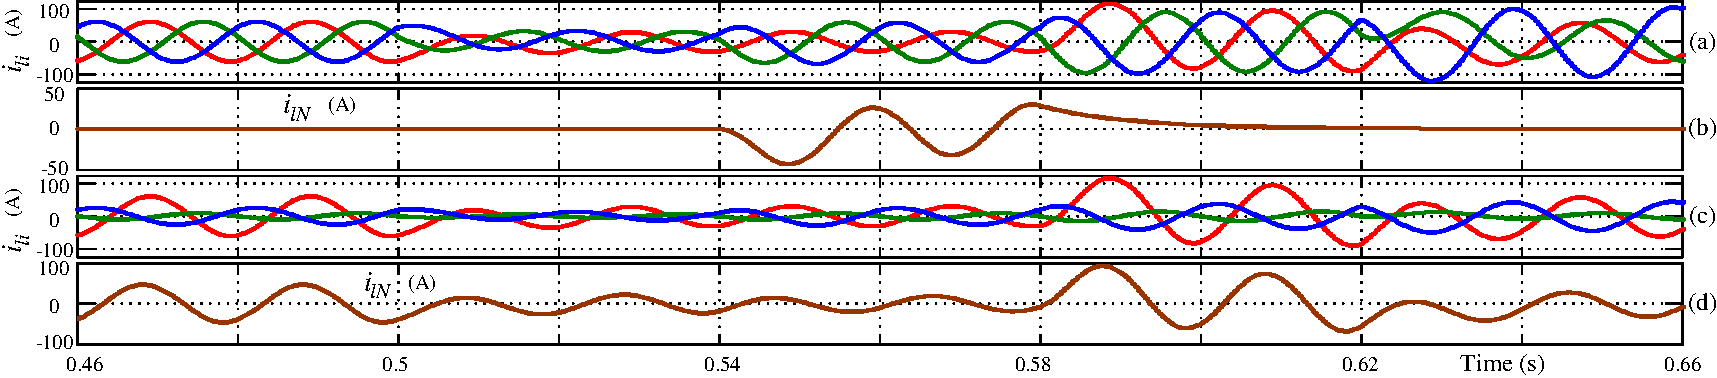
\includegraphics[scale=0.72	]{figures/Chapter_6/Mine/Res2.pdf}
	\caption{Simulation results of proposed SMC based four-leg DOC based UPQC-L during voltage anomalies with fundamental component: unbalanced swell ($V_{ga} = 1.1\,$pu), balanced swell ($V_{g} = 1.2\,$pu), unbalanced swell ($V_{ga} = 1.2\,$pu) and distorted grid} 
	\label{6.Res2} 
\end{sidewaysfigure}
\begin{sidewaysfigure}[]\centering
	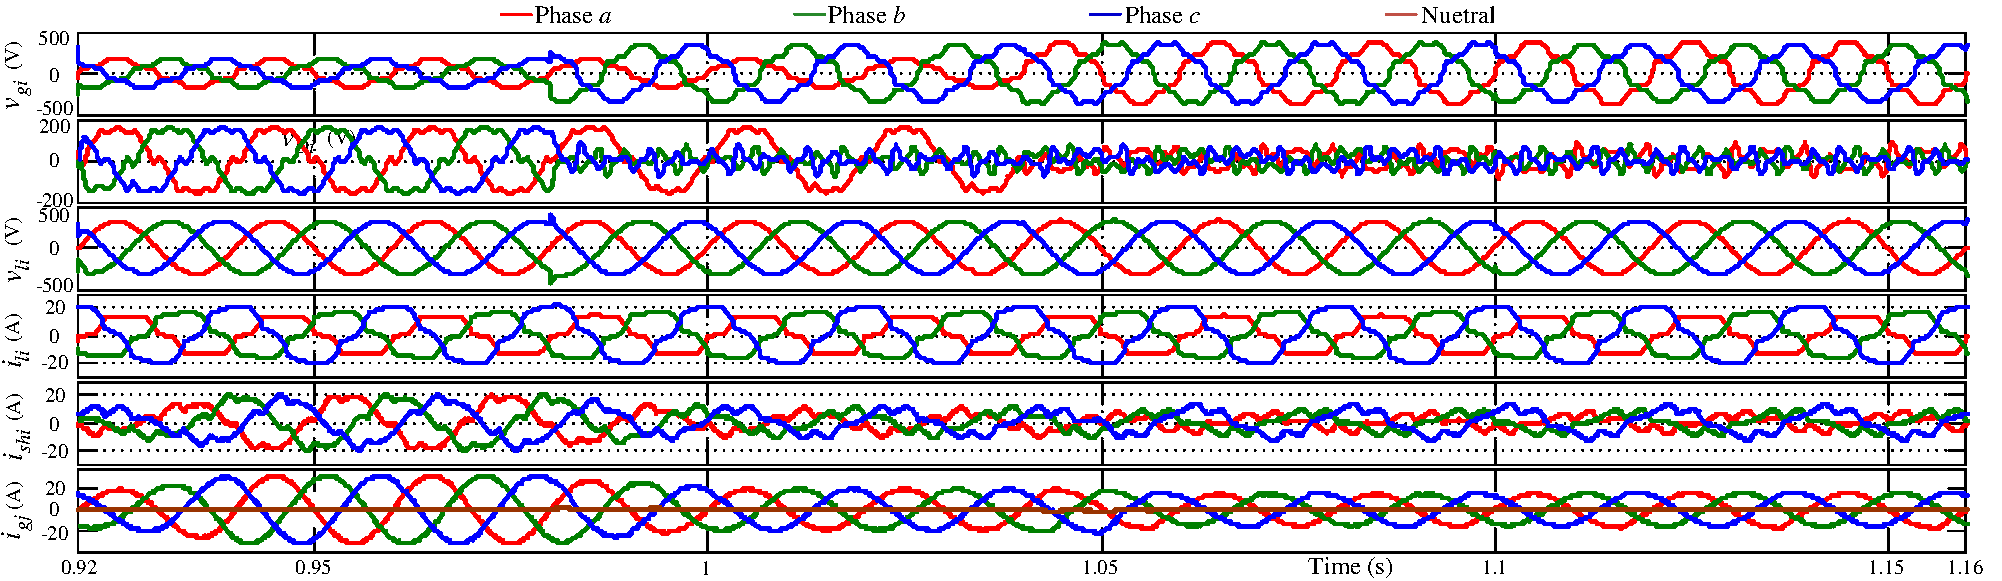
\includegraphics[scale=0.72	]{figures/Chapter_6/Mine/Res3.pdf}
	\caption{Simulation results of proposed SMC based four-leg DOC based UPQC-L during voltage anomalies with harmonic components: balanced sag ($V_g = 0.5\,$pu), unbalanced sag ($V_{ga} = 0.5\,$pu), balanced swell ($V_g = 1.1\,$pu), and unbalanced swell ($V_{ga} = 1.1\,$pu)} 
	\label{6.Res3} \vspace*{0.5cm}
	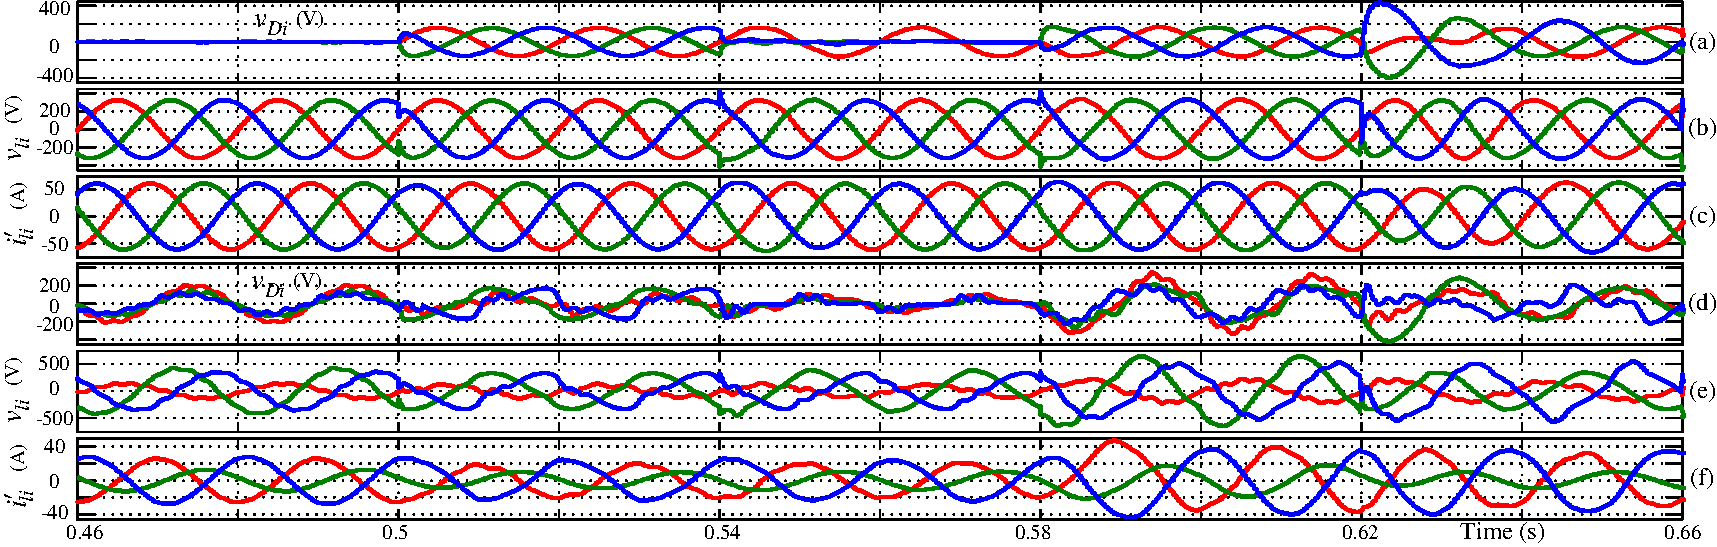
\includegraphics[scale=0.72	]{figures/Chapter_6/Mine/Res5.pdf}
	\caption{Simulation results of proposed SMC based four-leg DOC based UPQC-L during various voltage anomalies: reference and averaged NPVs of (a) DSTATCOM, and (b) DVR} 
	\label{6.Res5} 
\end{sidewaysfigure}

Figs.\,\ref{6.Res3}-\ref{6.Res4} display various system signals for voltage anomalies with harmonic components. In Fig.\,\ref{6.Res3}, a balanced voltage sag ($V_{g} = 0.5\, \si{pu}$), an unbalanced voltage sag in phase-$a$ ($V_{ga} = 0.5\, \si{pu}$), a balanced voltage swell ($V_{g} = 1.1\, \si{pu}$), and an unbalanced voltage swell in phase-$a$ ($V_{ga} = 1.1\, \si{pu}$) are considered at 0.92\,s, 0.98\,s, 1.04\,s and 1.1\,s, respectively. In Fig.\,\ref{6.Res4}, a balanced voltage swell ($V_{g} = 1.2\, \si{pu}$) and an unbalanced voltage swell in phase-$a$ ($V_{ga} = 1.2\, \si{pu}$) are considered at the time instants of 1.16\,s, and 1.22\,s, respectively.

\begin{figure}[]   
	\centering
	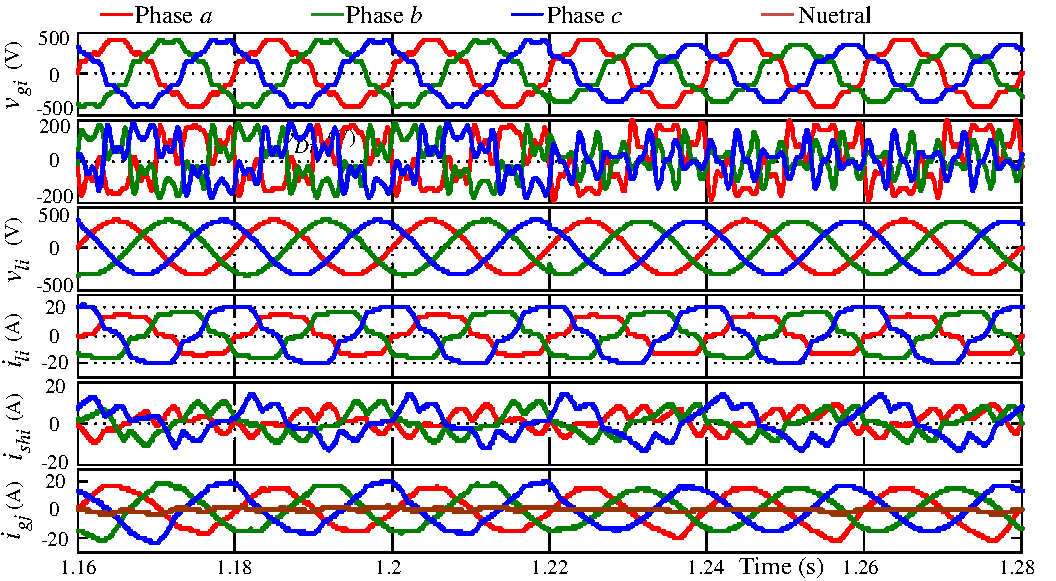
\includegraphics[scale=0.8]{figures/Chapter_6/Mine/Res4.pdf}
	\caption{Simulation results of proposed SMC based four-leg DOC based UPQC-L during voltage anomalies with harmonic components: balanced swell ($V_g = 1.2\,$pu), and unbalanced swell ($V_{ga} = 1.2\,$pu)}
	\label{6.Res4}
\end{figure}   

The simulation results demonstrate that the proposed control scheme exhibits fast response and effectively regulates the converter to fulfill the functionalities of both the DSTATCOM and DVR, namely ensuring load voltage regulation and load balancing. The current through the grid neutral ($i_{gN}$) is observed to be zero, indicating that the shunt terminals of the UPQC system supply the load neutral current. However, during a voltage swell of $1.2\,$pu, regardless of whether it is balanced or unbalanced, the compensator currents do not meet the required accuracy. This discrepancy arises due to the violation of the condition stated in \eqref{6.16}.

Additionally, the tracking performance of averaged neutral-point voltages (NPVs) with their reference values can be observed from Fig.\,\ref{6.Res5}. This demonstrates that the proposed scheme effectively controls both the NPVs, and the compensator voltages and currents.
\vspace*{2.5cm}

\section{SUMMARY}
The sliding mode control (SMC) scheme, previously introduced in the earlier chapters, is implemented in a dual-output converter-based UPQC-L system. Analytical expressions are derived for the reference neutral-point voltages (NPVs) of both the shunt and series terminals of the DOC-based UPQC-L system. Additionally, an expression is derived to determine the maximum value of voltage swell that the UPQC system can compensate. This limitation defines the range of voltage swell that can be effectively mitigated by the DOC-based UPQC-L system. To expand the compensation range for voltage swells, the DC-link voltage needs to be increased. 

To assess and verify the effectiveness of the proposed SMC scheme, a comprehensive simulation study is conducted. This study evaluates the performance of the control scheme under various scenarios, including both balanced and unbalanced upstream fault conditions. The simulation results provide insights into the behavior of the DOC based UPQC-L system and demonstrate the efficiency of the proposed SMC scheme in addressing power quality issues. 